% Created by tikzDevice version 0.7.0 on 2014-11-27 10:02:41
% !TEX encoding = UTF-8 Unicode
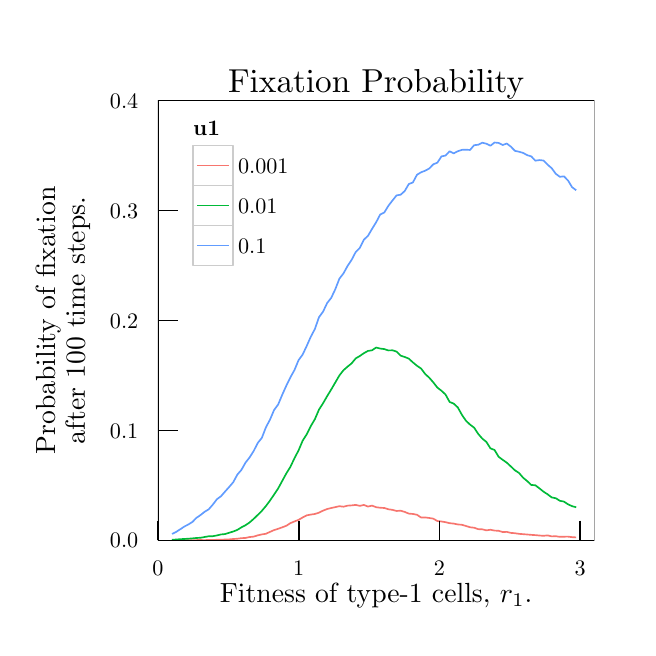
\begin{tikzpicture}[x=1pt,y=1pt]
\definecolor[named]{fillColor}{rgb}{1.00,1.00,1.00}
\path[use as bounding box,fill=fillColor,fill opacity=0.00] (0,0) rectangle (216.81,216.81);
\begin{scope}
\path[clip] (  0.00,  0.00) rectangle (216.81,216.81);
\definecolor[named]{drawColor}{rgb}{1.00,1.00,1.00}
\definecolor[named]{fillColor}{rgb}{1.00,1.00,1.00}

\path[draw=drawColor,line width= 0.6pt,line join=round,line cap=round,fill=fillColor] ( -0.00,  0.00) rectangle (216.81,216.81);
\end{scope}
\begin{scope}
\path[clip] ( 47.07, 31.56) rectangle (204.77,190.48);
\definecolor[named]{fillColor}{rgb}{1.00,1.00,1.00}

\path[fill=fillColor] ( 47.07, 31.56) rectangle (204.76,190.48);
\definecolor[named]{drawColor}{rgb}{0.97,0.46,0.43}

\path[draw=drawColor,line width= 0.6pt,line join=round] ( 52.15, 31.57) --
	( 53.63, 31.59) --
	( 55.10, 31.61) --
	( 56.58, 31.61) --
	( 58.05, 31.62) --
	( 59.53, 31.65) --
	( 61.00, 31.65) --
	( 62.48, 31.66) --
	( 63.95, 31.64) --
	( 65.43, 31.68) --
	( 66.90, 31.67) --
	( 68.38, 31.77) --
	( 69.86, 31.79) --
	( 71.33, 31.85) --
	( 72.81, 31.91) --
	( 74.28, 32.04) --
	( 75.76, 32.14) --
	( 77.23, 32.34) --
	( 78.71, 32.43) --
	( 80.18, 32.75) --
	( 81.66, 32.90) --
	( 83.13, 33.36) --
	( 84.61, 33.70) --
	( 86.08, 33.93) --
	( 87.56, 34.61) --
	( 89.03, 35.26) --
	( 90.51, 35.73) --
	( 91.98, 36.26) --
	( 93.46, 36.82) --
	( 94.93, 37.77) --
	( 96.41, 38.39) --
	( 97.89, 38.96) --
	( 99.36, 39.82) --
	(100.84, 40.59) --
	(102.31, 40.87) --
	(103.79, 41.09) --
	(105.26, 41.55) --
	(106.74, 42.29) --
	(108.21, 42.87) --
	(109.69, 43.24) --
	(111.16, 43.56) --
	(112.64, 43.90) --
	(114.11, 43.71) --
	(115.59, 44.09) --
	(117.06, 44.19) --
	(118.54, 44.36) --
	(120.01, 44.01) --
	(121.49, 44.35) --
	(122.96, 43.76) --
	(124.44, 44.11) --
	(125.92, 43.53) --
	(127.39, 43.33) --
	(128.87, 43.25) --
	(130.34, 42.79) --
	(131.82, 42.57) --
	(133.29, 42.17) --
	(134.77, 42.27) --
	(136.24, 41.83) --
	(137.72, 41.21) --
	(139.19, 41.09) --
	(140.67, 40.81) --
	(142.14, 39.82) --
	(143.62, 39.84) --
	(145.09, 39.64) --
	(146.57, 39.39) --
	(148.04, 38.54) --
	(149.52, 38.37) --
	(150.99, 38.12) --
	(152.47, 37.76) --
	(153.94, 37.61) --
	(155.42, 37.30) --
	(156.90, 37.18) --
	(158.37, 36.75) --
	(159.85, 36.28) --
	(161.32, 36.12) --
	(162.80, 35.60) --
	(164.27, 35.54) --
	(165.75, 35.16) --
	(167.22, 35.39) --
	(168.70, 35.08) --
	(170.17, 35.01) --
	(171.65, 34.55) --
	(173.12, 34.62) --
	(174.60, 34.25) --
	(176.07, 34.13) --
	(177.55, 33.90) --
	(179.02, 33.79) --
	(180.50, 33.67) --
	(181.97, 33.54) --
	(183.45, 33.44) --
	(184.93, 33.30) --
	(186.40, 33.19) --
	(187.88, 33.35) --
	(189.35, 32.99) --
	(190.83, 33.05) --
	(192.30, 32.82) --
	(193.78, 32.88) --
	(195.25, 32.89) --
	(196.73, 32.71) --
	(198.20, 32.62);
\definecolor[named]{drawColor}{rgb}{0.00,0.73,0.22}

\path[draw=drawColor,line width= 0.6pt,line join=round] ( 52.15, 31.76) --
	( 53.63, 31.85) --
	( 55.10, 31.98) --
	( 56.58, 32.05) --
	( 58.05, 32.15) --
	( 59.53, 32.27) --
	( 61.00, 32.41) --
	( 62.48, 32.49) --
	( 63.95, 32.77) --
	( 65.43, 33.03) --
	( 66.90, 33.06) --
	( 68.38, 33.33) --
	( 69.86, 33.69) --
	( 71.33, 33.83) --
	( 72.81, 34.30) --
	( 74.28, 34.75) --
	( 75.76, 35.33) --
	( 77.23, 36.25) --
	( 78.71, 37.01) --
	( 80.18, 38.02) --
	( 81.66, 39.31) --
	( 83.13, 40.73) --
	( 84.61, 42.20) --
	( 86.08, 43.95) --
	( 87.56, 45.91) --
	( 89.03, 48.10) --
	( 90.51, 50.32) --
	( 91.98, 53.02) --
	( 93.46, 55.74) --
	( 94.93, 58.10) --
	( 96.41, 61.25) --
	( 97.89, 64.06) --
	( 99.36, 67.56) --
	(100.84, 69.89) --
	(102.31, 72.84) --
	(103.79, 75.35) --
	(105.26, 78.79) --
	(106.74, 81.10) --
	(108.21, 83.65) --
	(109.69, 86.07) --
	(111.16, 88.60) --
	(112.64, 91.14) --
	(114.11, 93.03) --
	(115.59, 94.31) --
	(117.06, 95.52) --
	(118.54, 97.31) --
	(120.01, 98.16) --
	(121.49, 99.19) --
	(122.96,100.00) --
	(124.44,100.23) --
	(125.92,101.23) --
	(127.39,100.85) --
	(128.87,100.67) --
	(130.34,100.18) --
	(131.82,100.23) --
	(133.29, 99.76) --
	(134.77, 98.29) --
	(136.24, 97.82) --
	(137.72, 97.21) --
	(139.19, 95.87) --
	(140.67, 94.64) --
	(142.14, 93.67) --
	(143.62, 91.68) --
	(145.09, 90.34) --
	(146.57, 88.64) --
	(148.04, 86.75) --
	(149.52, 85.62) --
	(150.99, 84.24) --
	(152.47, 81.56) --
	(153.94, 80.96) --
	(155.42, 79.59) --
	(156.90, 76.93) --
	(158.37, 74.77) --
	(159.85, 73.38) --
	(161.32, 72.28) --
	(162.80, 70.02) --
	(164.27, 68.32) --
	(165.75, 67.12) --
	(167.22, 64.79) --
	(168.70, 64.20) --
	(170.17, 61.76) --
	(171.65, 60.65) --
	(173.12, 59.63) --
	(174.60, 58.25) --
	(176.07, 56.86) --
	(177.55, 55.91) --
	(179.02, 54.19) --
	(180.50, 52.97) --
	(181.97, 51.58) --
	(183.45, 51.45) --
	(184.93, 50.33) --
	(186.40, 49.15) --
	(187.88, 48.19) --
	(189.35, 47.07) --
	(190.83, 46.78) --
	(192.30, 45.85) --
	(193.78, 45.56) --
	(195.25, 44.57) --
	(196.73, 43.90) --
	(198.20, 43.51);
\definecolor[named]{drawColor}{rgb}{0.38,0.61,1.00}

\path[draw=drawColor,line width= 0.6pt,line join=round] ( 52.15, 33.87) --
	( 53.63, 34.59) --
	( 55.10, 35.54) --
	( 56.58, 36.53) --
	( 58.05, 37.28) --
	( 59.53, 38.21) --
	( 61.00, 39.70) --
	( 62.48, 40.71) --
	( 63.95, 41.88) --
	( 65.43, 42.78) --
	( 66.90, 44.47) --
	( 68.38, 46.41) --
	( 69.86, 47.50) --
	( 71.33, 49.19) --
	( 72.81, 50.84) --
	( 74.28, 52.56) --
	( 75.76, 55.31) --
	( 77.23, 57.01) --
	( 78.71, 59.63) --
	( 80.18, 61.50) --
	( 81.66, 63.83) --
	( 83.13, 66.73) --
	( 84.61, 68.57) --
	( 86.08, 72.38) --
	( 87.56, 75.16) --
	( 89.03, 78.63) --
	( 90.51, 80.65) --
	( 91.98, 84.15) --
	( 93.46, 87.44) --
	( 94.93, 90.44) --
	( 96.41, 93.11) --
	( 97.89, 96.67) --
	( 99.36, 98.68) --
	(100.84,101.82) --
	(102.31,105.13) --
	(103.79,107.95) --
	(105.26,112.17) --
	(106.74,114.20) --
	(108.21,117.30) --
	(109.69,119.18) --
	(111.16,122.30) --
	(112.64,126.11) --
	(114.11,128.01) --
	(115.59,130.70) --
	(117.06,132.92) --
	(118.54,135.75) --
	(120.01,137.21) --
	(121.49,140.21) --
	(122.96,141.57) --
	(124.44,144.10) --
	(125.92,146.50) --
	(127.39,149.30) --
	(128.87,150.03) --
	(130.34,152.44) --
	(131.82,154.36) --
	(133.29,156.20) --
	(134.77,156.45) --
	(136.24,157.77) --
	(137.72,160.31) --
	(139.19,160.87) --
	(140.67,163.65) --
	(142.14,164.55) --
	(143.62,165.11) --
	(145.09,165.91) --
	(146.57,167.43) --
	(148.04,168.02) --
	(149.52,170.29) --
	(150.99,170.59) --
	(152.47,172.15) --
	(153.94,171.38) --
	(155.42,172.17) --
	(156.90,172.66) --
	(158.37,172.71) --
	(159.85,172.62) --
	(161.32,174.34) --
	(162.80,174.50) --
	(164.27,175.24) --
	(165.75,174.87) --
	(167.22,174.14) --
	(168.70,175.31) --
	(170.17,175.16) --
	(171.65,174.40) --
	(173.12,174.95) --
	(174.60,173.81) --
	(176.07,172.30) --
	(177.55,171.98) --
	(179.02,171.55) --
	(180.50,170.74) --
	(181.97,170.30) --
	(183.45,168.74) --
	(184.93,168.97) --
	(186.40,168.80) --
	(187.88,167.30) --
	(189.35,166.03) --
	(190.83,164.01) --
	(192.30,162.92) --
	(193.78,163.09) --
	(195.25,161.59) --
	(196.73,159.15) --
	(198.20,158.07);
\definecolor[named]{drawColor}{rgb}{0.00,0.00,0.00}

\path[draw=drawColor,line width= 0.6pt,line join=round,line cap=round] ( 47.07, 31.56) rectangle (204.76,190.48);
\end{scope}
\begin{scope}
\path[clip] (  0.00,  0.00) rectangle (216.81,216.81);
\definecolor[named]{drawColor}{rgb}{0.00,0.00,0.00}

\node[text=drawColor,anchor=base east,inner sep=0pt, outer sep=0pt, scale=  0.80] at ( 39.95, 28.80) {0.0};

\node[text=drawColor,anchor=base east,inner sep=0pt, outer sep=0pt, scale=  0.80] at ( 39.95, 68.53) {0.1};

\node[text=drawColor,anchor=base east,inner sep=0pt, outer sep=0pt, scale=  0.80] at ( 39.95,108.26) {0.2};

\node[text=drawColor,anchor=base east,inner sep=0pt, outer sep=0pt, scale=  0.80] at ( 39.95,147.99) {0.3};

\node[text=drawColor,anchor=base east,inner sep=0pt, outer sep=0pt, scale=  0.80] at ( 39.95,187.72) {0.4};
\end{scope}
\begin{scope}
\path[clip] (  0.00,  0.00) rectangle (216.81,216.81);
\definecolor[named]{drawColor}{rgb}{0.00,0.00,0.00}

\path[draw=drawColor,line width= 0.6pt,line join=round] ( 54.18, 31.56) --
	( 47.07, 31.56);

\path[draw=drawColor,line width= 0.6pt,line join=round] ( 54.18, 71.29) --
	( 47.07, 71.29);

\path[draw=drawColor,line width= 0.6pt,line join=round] ( 54.18,111.02) --
	( 47.07,111.02);

\path[draw=drawColor,line width= 0.6pt,line join=round] ( 54.18,150.75) --
	( 47.07,150.75);

\path[draw=drawColor,line width= 0.6pt,line join=round] ( 54.18,190.48) --
	( 47.07,190.48);
\end{scope}
\begin{scope}
\path[clip] (  0.00,  0.00) rectangle (216.81,216.81);
\definecolor[named]{drawColor}{rgb}{0.00,0.00,0.00}

\path[draw=drawColor,line width= 0.6pt,line join=round] ( 47.07, 38.67) --
	( 47.07, 31.56);

\path[draw=drawColor,line width= 0.6pt,line join=round] ( 97.94, 38.67) --
	( 97.94, 31.56);

\path[draw=drawColor,line width= 0.6pt,line join=round] (148.81, 38.67) --
	(148.81, 31.56);

\path[draw=drawColor,line width= 0.6pt,line join=round] (199.68, 38.67) --
	(199.68, 31.56);
\end{scope}
\begin{scope}
\path[clip] (  0.00,  0.00) rectangle (216.81,216.81);
\definecolor[named]{drawColor}{rgb}{0.00,0.00,0.00}

\node[text=drawColor,anchor=base,inner sep=0pt, outer sep=0pt, scale=  0.80] at ( 47.07, 18.93) {0};

\node[text=drawColor,anchor=base,inner sep=0pt, outer sep=0pt, scale=  0.80] at ( 97.94, 18.93) {1};

\node[text=drawColor,anchor=base,inner sep=0pt, outer sep=0pt, scale=  0.80] at (148.81, 18.93) {2};

\node[text=drawColor,anchor=base,inner sep=0pt, outer sep=0pt, scale=  0.80] at (199.68, 18.93) {3};
\end{scope}
\begin{scope}
\path[clip] (  0.00,  0.00) rectangle (216.81,216.81);
\definecolor[named]{drawColor}{rgb}{0.00,0.00,0.00}

\node[text=drawColor,anchor=base,inner sep=0pt, outer sep=0pt, scale=  1.00] at (125.92,  9.03) {Fitness of type-1 cells, $r_1$.};
\end{scope}
\begin{scope}
\path[clip] (  0.00,  0.00) rectangle (216.81,216.81);
\definecolor[named]{drawColor}{rgb}{0.00,0.00,0.00}

\node[text=drawColor,rotate= 90.00,anchor=base,inner sep=0pt, outer sep=0pt, scale=  1.00] at (  9.90,111.02) {Probability of fixation };

\node[text=drawColor,rotate= 90.00,anchor=base,inner sep=0pt, outer sep=0pt, scale=  1.00] at ( 20.70,111.02) {  after 100 time steps.};
\end{scope}
\begin{scope}
\path[clip] (  0.00,  0.00) rectangle (216.81,216.81);
\definecolor[named]{fillColor}{rgb}{1.00,1.00,1.00}

\path[fill=fillColor] ( 55.52,126.59) rectangle ( 98.54,187.62);
\end{scope}
\begin{scope}
\path[clip] (  0.00,  0.00) rectangle (216.81,216.81);
\definecolor[named]{drawColor}{rgb}{0.00,0.00,0.00}

\node[text=drawColor,anchor=base west,inner sep=0pt, outer sep=0pt, scale=  0.80] at ( 59.79,177.83) {\bfseries u1};
\end{scope}
\begin{scope}
\path[clip] (  0.00,  0.00) rectangle (216.81,216.81);
\definecolor[named]{drawColor}{rgb}{0.80,0.80,0.80}
\definecolor[named]{fillColor}{rgb}{1.00,1.00,1.00}

\path[draw=drawColor,line width= 0.6pt,line join=round,line cap=round,fill=fillColor] ( 59.79,159.76) rectangle ( 74.24,174.22);
\end{scope}
\begin{scope}
\path[clip] (  0.00,  0.00) rectangle (216.81,216.81);
\definecolor[named]{drawColor}{rgb}{0.97,0.46,0.43}

\path[draw=drawColor,line width= 0.6pt,line join=round] ( 61.23,166.99) -- ( 72.80,166.99);
\end{scope}
\begin{scope}
\path[clip] (  0.00,  0.00) rectangle (216.81,216.81);
\definecolor[named]{drawColor}{rgb}{0.80,0.80,0.80}
\definecolor[named]{fillColor}{rgb}{1.00,1.00,1.00}

\path[draw=drawColor,line width= 0.6pt,line join=round,line cap=round,fill=fillColor] ( 59.79,145.31) rectangle ( 74.24,159.76);
\end{scope}
\begin{scope}
\path[clip] (  0.00,  0.00) rectangle (216.81,216.81);
\definecolor[named]{drawColor}{rgb}{0.00,0.73,0.22}

\path[draw=drawColor,line width= 0.6pt,line join=round] ( 61.23,152.54) -- ( 72.80,152.54);
\end{scope}
\begin{scope}
\path[clip] (  0.00,  0.00) rectangle (216.81,216.81);
\definecolor[named]{drawColor}{rgb}{0.80,0.80,0.80}
\definecolor[named]{fillColor}{rgb}{1.00,1.00,1.00}

\path[draw=drawColor,line width= 0.6pt,line join=round,line cap=round,fill=fillColor] ( 59.79,130.86) rectangle ( 74.24,145.31);
\end{scope}
\begin{scope}
\path[clip] (  0.00,  0.00) rectangle (216.81,216.81);
\definecolor[named]{drawColor}{rgb}{0.38,0.61,1.00}

\path[draw=drawColor,line width= 0.6pt,line join=round] ( 61.23,138.08) -- ( 72.80,138.08);
\end{scope}
\begin{scope}
\path[clip] (  0.00,  0.00) rectangle (216.81,216.81);
\definecolor[named]{drawColor}{rgb}{0.00,0.00,0.00}

\node[text=drawColor,anchor=base west,inner sep=0pt, outer sep=0pt, scale=  0.80] at ( 76.05,164.24) {0.001};
\end{scope}
\begin{scope}
\path[clip] (  0.00,  0.00) rectangle (216.81,216.81);
\definecolor[named]{drawColor}{rgb}{0.00,0.00,0.00}

\node[text=drawColor,anchor=base west,inner sep=0pt, outer sep=0pt, scale=  0.80] at ( 76.05,149.78) {0.01};
\end{scope}
\begin{scope}
\path[clip] (  0.00,  0.00) rectangle (216.81,216.81);
\definecolor[named]{drawColor}{rgb}{0.00,0.00,0.00}

\node[text=drawColor,anchor=base west,inner sep=0pt, outer sep=0pt, scale=  0.80] at ( 76.05,135.33) {0.1};
\end{scope}
\begin{scope}
\path[clip] (  0.00,  0.00) rectangle (216.81,216.81);
\definecolor[named]{drawColor}{rgb}{0.00,0.00,0.00}

\node[text=drawColor,anchor=base,inner sep=0pt, outer sep=0pt, scale=  1.20] at (125.92,193.49) {Fixation Probability};
\end{scope}
\end{tikzpicture}
